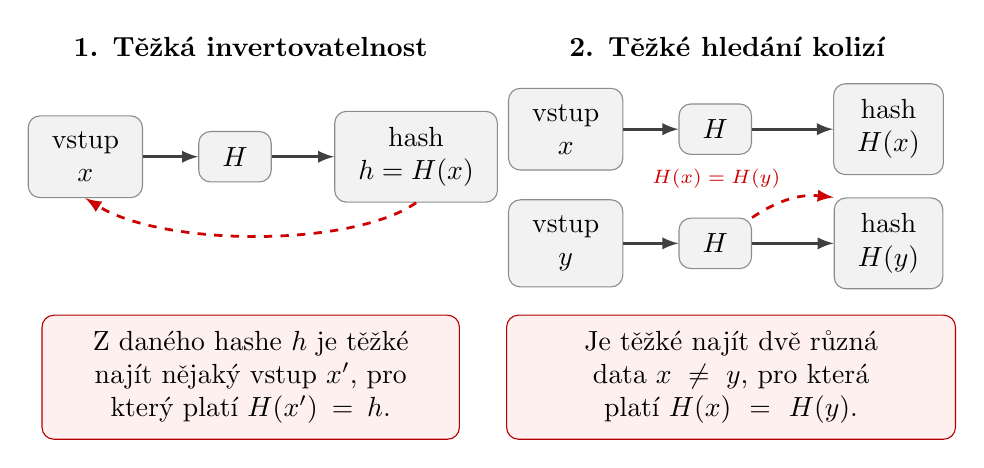
\begin{tikzpicture}[
    x=1cm, y=1cm,
    >=latex,
    arrow/.style={->, >=latex, line width=1pt, draw=black!75},
    hard/.style={->, >=latex, dashed, line width=1pt, draw=red!80!black},
    box/.style={
        rounded corners=1.5mm,
        draw=black!45,
        fill=black!5,
        inner xsep=3mm,
        inner ysep=2mm,
        align=center
    },
    req/.style={
        rounded corners=1.5mm,
        draw=red!70!black,
        fill=red!6,
        inner xsep=3mm,
        inner ysep=2mm,
        align=center
    }
]

    %------------------------------------------------
    % 1. Těžká invertovatelnost
    %------------------------------------------------
    \node[font=\bfseries] at (-3.1,2.2) {1. Těžká invertovatelnost};

    \node[box] (in1) at (-5.2,0.8) {vstup\\ $x$};
    \node[box] (H1)  at (-3.3,0.8) {$H$};
    \node[box] (out1) at (-1.0,0.8) {hash\\ $h=H(x)$};

    \draw[arrow] (in1.east) -- (H1.west);
    \draw[arrow] (H1.east) -- (out1.west);

    \draw[hard] (out1.south) .. controls (-1.8,-0.35) and (-4.2,-0.35) .. (in1.south);
    \node[req, text width=4.7cm] at (-3.1,-2.0)
    {Z daného hashe $h$ je těžké najít nějaký vstup $x'$, pro který platí $H(x')=h$.};

    %------------------------------------------------
    % 2. Těžké hledání kolizí
    %------------------------------------------------
    \node[font=\bfseries] at (2.95,2.2) {2. Těžké hledání kolizí};

    \node[box] (x2) at (0.9,1.15) {vstup\\ $x$};
    \node[box] (y2) at (0.9,-0.3)  {vstup\\ $y$};

    \node[box] (Hx) at (2.8,1.15) {$H$};
    \node[box] (Hy) at (2.8,-0.3)  {$H$};

    \node[box] (hx) at (5.0,1.15) {hash\\ $H(x)$};
    \node[box] (hy) at (5.0,-0.3)  {hash\\ $H(y)$};

    \draw[arrow] (x2.east) -- (Hx.west);
    \draw[arrow] (y2.east) -- (Hy.west);
    \draw[arrow] (Hx.east) -- (hx.west);
    \draw[arrow] (Hy.east) -- (hy.west);

    \node[req, text width=5.1cm] at (3.0,-2.0)
    {Je těžké najít dvě různá data $x\neq y$, pro která platí $H(x)=H(y)$.};

    % zvýraznění kolize
    \draw[hard] (Hy.north east) to[bend left=20] node[font=\scriptsize, text=red!80!black,midway,above left] {$H(x)=H(y)$} (hy.north west);

\end{tikzpicture}
